\documentclass[11pt]{article}
\usepackage{tdt13}
\usepackage[norsk,british]{babel}             % Correct Norwegian and English hyphenation
\usepackage[utf8]{inputenc}                     % Allow for non-ASCII input
\usepackage[T1]{fontenc}                         % Use rich fonts
\usepackage{times}
\usepackage{latexsym}
\usepackage{csquotes}

%%%%%%%%%%%%%%%%%%%%%%%%%%%%%%%%%%%%%%%%%%%%%%%%%%%%%
% Hyperlinks, you can choose different colours for different types of links; the defult colours are as below
\usepackage[colorlinks]{hyperref}
\hypersetup{
    linkcolor=black,	% internal cross-references; default red
    urlcolor=blue,	% default magenta
    citecolor=black,	% default green
   }
\urlstyle{same}	% if you want links in the same style as the rest of the text; default is typewriter style
\usepackage{doi}

%%%%%%%%%%%%%%%%%%%%%%%%%%%%%%%%%%%%%%%%%%%%%%%%%%%%%
% Graphics, tables and figures
\usepackage{graphicx}                           
\usepackage[table]{xcolor}
\usepackage{colortbl}
\usepackage{tcolorbox}
\usepackage{framed}
\usepackage{tabularx}
\usepackage{multicol}
\usepackage{multirow}
\usepackage{rotating}
\usepackage{array}
\usepackage{supertabular}
\usepackage{hhline}
\usepackage{subcaption}

% nicer table dividers
\newcommand\tabletop{\hline\noalign{\smallskip}}
\newcommand\tablemid{\noalign{\smallskip}\hline\noalign{\smallskip}}
\newcommand\tablebot{\noalign{\smallskip}\hline}

% only needed if you want to pgfplots to draw figures
%\usepackage{tikzsymbols}
%\usepackage{pgfplots}

%%%%%%%%%%%%%%%%%%%%%%%%%%%%%%%%%%%%%%%%%%%%%%%%%%%%%
% comments and notes, useful while working on a draft - change the option 'draft' to 'disable' in the final version
\usepackage[draft]{todonotes}
\usepackage{verbatim}     % allow for longer comments

%%%%%%%%%%%%%%%%%%%%%%%%%%%%%%%%%%%%%%%%%%%%%%%%%%%%%
% BIBLIOGRAPHY STUFF

% \usepackage[round]{natbib}

\usepackage[backend=biber,
            bibstyle=apa,
            citestyle=authoryear,
            natbib=true,
            url=false,
            doi=false,
            hyperref=true,
            apamaxprtauth=99,
            maxcitenames=2,
            language=british,
            uniquelist=false,
            ]{biblatex}         

% Bibliography (+ hacks)
\addbibresource{bib/bibliography.bib}
\DeclareLanguageMapping{british}{british-apa}
\setlength\bibitemsep{2\itemsep}
\patchcmd{\bibsetup}{\interlinepenalty=5000}{\interlinepenalty=10000}{}{}
\let\citep\parencite
\let\cite\textcite
% Make the whole cite a hyperref
\DeclareCiteCommand{\textcite}
{\boolfalse{cbx:parens}}
{\usebibmacro{citeindex}%
    \printtext[bibhyperref]{\usebibmacro{textcite}}}
{\ifbool{cbx:parens}
    {\bibcloseparen\global\boolfalse{cbx:parens}}
    {}%
    \multicitedelim}
{\usebibmacro{textcite:postnote}}
\DeclareCiteCommand{\parencite}[\mkbibparens]
{\usebibmacro{prenote}}
{\usebibmacro{citeindex}%
    \printtext[bibhyperref]{\usebibmacro{cite}}}
{\multicitedelim}
{\usebibmacro{postnote}}

%%%%%%%%%%%%%%%%%%%%%%%%%%%%%%%%%%%%%%%%%%%%%%%%%%%%%
% HYPHENATION DEFINITIONS

\usepackage{hyphenat}

% add correct hyphenations as needed
\hyphenation{hash-tag Sem-Eval}
\hyphenation{cyber-bully cyber-bullying}

% Acronym stuff
\usepackage[
nonumberlist, 			% if you don't want to show pagenumbers 
toc, 					% entry in the table of contents; can be left out
acronym] 				% create a list of abbreviations
{glossaries}
\usepackage[acronym]{glossaries}
\makeglossaries
\loadglsentries[main]{glossary}
%%%%%%%%%%%%%%%%%%%%%%%%%%%%%%%%%%%%%%%%%%%%%%%%%%%%%

\title{Geolocation Prediction from Jodel and Twitter Messages}

\author{Karl Oskar Magnus Holm \\
  Engineering Science and ICT - Department of Geomatics / 2023 \\
  {\tt koholm@stud.ntnu.no} \\}

\date{Report in TDT13, NTNU, \today}

\begin{document}
\maketitle


\begin{abstract}
    \begin{comment}
    This paper provides a template for writing a Project Report in TDT13, Advanced Text Analytics and Language Understanding.
    The document itself conforms to its own specifications and is thus an example of what your manuscript should look like.
    The template does not form a compulsory style that you are obliged to use, but rather provides a common starting point for all students.
    For a given report, tuning of the template may still be required, depending on the nature of the report and the author's writing style.
    Such tuning might involve moving a section to a subsection or vice versa, or removing or adding sections and subsections.

    Note that the template contains a lot of examples of how to write different parts of the report
    as well as how to cite authors and how to use LaTeX and BibTeX.
    Some of those examples might only be clear if you actually look at the LaTeX source itself.

    The abstract is your sales pitch which encourages people to read your work,
    but unlike sales it should be realistic with respect to the contributions of the work.
    It should include:
    \begin{itemize}
        \item what the research topic is,
        \item the research approach(es) applied, and
        \item contributions.
    \end{itemize}

    The abstract should not exceed 200 words.
    Do not include lists, tables or figures.
    Avoid abbreviations and references.
    \end{comment}
\end{abstract}

\glsaddall

\section{Introduction}
\label{sec:Introduction}

\begin{comment}
Each section should start with an introduction before its subsections begin.
Sections with just one sub-section should be avoided.
Think carefully about section titles as each title should convey the meaning of the contents of the section.

In all sections it is important to write clearly and concisely.
Avoid repetitions and if needed refer back to the original discussion or presentation.
Each new section, subsection or paragraph should provide the reader with new information and be written in your own words.
Avoid direct quotes. If you use direct quotes, unless the quote itself is very significant,
you are conveying to the reader that you are unable to express this discussion or fact yourself.
Such direct quotes also break the flow of the language (yours to someone else's).

Manuscripts must be in single-column format. {\bf Type single-spaced.}
You may prepare your PDF files using any word processor,
but templates are only provided for \LaTeX\ and Microsoft Word.
For the production of the electronic manuscript you must use Adobe's Portable Document Format (PDF).
PDF files are usually produced from \LaTeX\ using the \textit{pdflatex} command.
If your version of \LaTeX\ produces Postscript files, you can convert these into PDF using \textit{ps2pdf} or \textit{dvipdf}.
On Windows, you can also use Adobe Distiller to generate PDF, or the print to  or save to PDF functions.

For reasons of uniformity, Adobe's {\bf Times Roman} font should be used,
with 11pt for the text, 12pt for section titles, and 15pt for the title of the report.
If Times Roman is unavailable, use {\bf Computer Modern Roman} (\LaTeX2e{}'s default).
Note that the latter is about 10\% less dense than Adobe's Times Roman font.
Please make sure that your PDF file includes all the necessary fonts (especially tree diagrams, symbols, and fonts for non-Latin characters).
When you print or create the PDF file, there is usually an option in your printer setup to include none, all or just non-standard fonts.
Please make sure that you select the option of including ALL the fonts.

The section `Introduction' should give the background and motivation for the work, that is,
it should state where your project is situated in the field and what the key driving forces motivating this research are.
However, keep that text brief, as it will be further extended in Section~\ref{sec:related_work}, presenting the state-of-the-art.
Your goal/objective should be possible to describe in a single sentence.
In the text after it you can expand on this sentence to clarify what is meant by the short goal description.
The goal of your work is what you are trying to achieve.
Potentially, how well the goal has been met is a theme that you should return to towards the end of the report (so in Section~\ref{sec:Conclusion} and possibly in Section~\ref{sec:Discussion} as well).

The introduction can also briefly describe what methodology you will apply to reach the goal and the reasons for this choice of research methodology.
It can furthermore provide a brief summary of the main contributions of the work,
and should provide the reader with an overview of what is coming in the next sections.
You want to say more than what is explicit in the section names, if possible, but still keep the description short and to the point.
\end{comment}

This project is based on the shared task on \gls{acr:smg} from VarDial 2020 and 2021 (seventh and eighth edition, respectively), the Workshop on \gls{acr:nlp} for Similar Languages, Varieties and Dialects \citep{gamanReportVarDialEvaluation2020, chakravarthiFindingsVarDialEvaluation2021}. The aim of the task differs somewhat from the most common types of \gls{acr:nlp} VarDial tasks, where the goal typically is to choose from a finite set of variety labels \citep[1]{scherrerSocialMediaVariety2021}. Here, the goal is to predict a set of scalars, namely the latitude and longitude from which a social media post was posted. This VarDial task stayed the same from 2020 to 2021, including three language areas: the Bosnian-Croatian-Montenegrin-Serbian language area, the German language area (Germany and Austria in this case), and the German-speaking Switzerland.

This project is limited to the latter of these language areas, that is, the German-speaking Switzerland. Reasons for this include the limited time scope of the task, and having to share the necessary computing resources with fellow students at the department. The goal is to try and recreate the results of \cite{scherrerHeLjuVarDial20202020} who used a \acrshort{acr:bert}-based classifier, making it a double regression task. I focus on the \citeyear{scherrerHeLjuVarDial20202020} dataset because there were a lot more submissions this year as opposed to in \citeyear{scherrerSocialMediaVariety2021}, due to the short time between the announcement of the shared task and the submission deadline \citep[6]{chakravarthiFindingsVarDialEvaluation2021}.

The reason for picking the task on the German-speaking Switzerland is its similarities to the dialectal landscape of Norway. \cite[14]{roynelandDialectsNorwayCatching2009} writes that "dialects in Norway have had and still have a much stronger position than dialects ... in most of Europe, except for the German-speaking part of Switzerland.". I therefore find it reasonable to assume that a method which works well on the Swiss dataset could also perform well on a Norwegian dataset. Unfortunately, I was unable to find a suitable Norwegian dataset, and creating one proved too difficult and time-consuming to be worthwhile, considering the time horizon of the project.

Code and data used to develop models is available at \texttt{\url{https://github.com/oskarhlm/TDT13}}.
\section{Background}
%OR: \section{Tools and Methods}
\label{sec:background}

The background's depth and breadth depend on the depth needed to understand your project.
It is not a place to just write about everything you know that is vaguely connected to your project. 
The theory is here to help the readers that do not know the theoretical basis of your work, so that they 
can gain sufficient understanding to understand your contributions. In particular, the theory section provides 
an opportunity to introduce terminology that can later be used without disturbing the text with a definition.  

When introducing techniques or results, always reference the source. 
Be careful to reference the original contributor of a technique and not just someone who happens to use the technique.%
\footnote{But always make sure that you have read the work you are citing --- if not, cite someone who has!}
For results relevant to your work, 
you would want to look particularly at newer results so that you have referenced the most up-to-date work in your area. 
If you do not have the source handy when writing, mark in the text that a reference is needed and add it later. \todo{add reference} 
Web pages are not reliable sources --- they might be there one day and removed the next; and thus should be avoided, if possible. 
A verbal discussion is not a source and should normally not be referenced.  
The bulk of citations in the report will appear in Section~\ref{sec:related_work}. 
However, you will often need to introduce some terminology and key citations already in this section. 
%
You can cite a paper in the following manner (and several other versions, 
see the \verb!natbib! package documentation):

\begin{itemize}
\item when referring to authors:\\
 \citet{Authorson;Bobsen:10} stated something rather nice.
\item to cite indirectly: \\
 Papers should be written nicely \citep{Authorson;Bobsen:10}
{\em or\/}\\
In \cite{Authorson;Bobsen:10}, a less detailed template was presented.
\item To just cite the authors: \\
\citeauthor{Authorson;Bobsen:10} wrote a nice paper.
Or just the year: \citeyear{Authorson;Bobsen:10}.
\item You can even cite specific pages: \citet[p. 3]{Authorson;Bobsen:10}.
\end{itemize}

You should obviously always cite your teacher's work \citep{BenyonEA:13}, 
even if it is completely irrelevant \citep{Das;Gamback:13a} or very old \citep{AlshawiEA:91b}.
Digging up an even older book can also appear impressive \citep{Diderichsen:57}.
(Or? ;-)

\subsection{Introducing Figures}

\begin{figure}[t!]
\centering
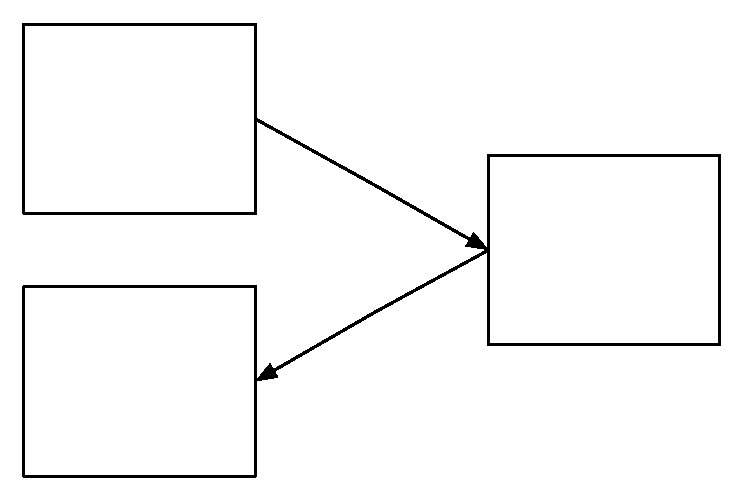
\includegraphics[width=0.5\columnwidth]{figs/figure1.pdf}
\caption[Boxes and arrows are nice]{Boxes and arrows are nice (adapted from \citealp{Authorson;Bobsen:10}, with permission)}
\label{fig:BoxesAndArrowsAreNice}
\end{figure}

Remember that when you borrow figures you should always credit the original author --- such as 
Figure~\ref{fig:BoxesAndArrowsAreNice} (adapted from \citealp{Authorson;Bobsen:10}),
as well as state that you have permission to reprint it (e.g., if it is published under a Creative Commons License,
or if you have gained explicit permission from the author). 

Do not just put the figure in and leave it to the reader to try to understand what the figure is. 
The figure should be included to convey a message and you need to help the reader to understand the message 
intended by explaining the figure in the text. Hence {\bf all} figures and tables should always be referenced in the text.
There will often be specific parts of a figure or table that you want the reader to pay special attention to (and that you
discuss in more detail in the text). It is helpful if you mark those parts clearly (e.g., by circling them, pointing them out
with arrows, using different colours and fonts, etc.)

It is good practice to add a note about a missing figure in the text,
such as the completely amazing stuff that will appear in Figure~\ref{fig:AmazingFigure}.

Narrow graphics together with the single-column format may lead to large empty spaces.
If you have multiple graphics with related content, it may be preferable to combine them in one graphic.
You can identify the sub-graphics with sub-captions below the sub-graphics numbered (a), (b), (c) etc., and using 9pt text.
The \LaTeX\ packages wrapfig, subfig, subtable and/or subcaption may be useful.

\begin{figure}[t!]
\centering
\missingfigure{Here we will add an amazing figure explaining it all}
\caption{A missing figure}
\label{fig:AmazingFigure}
\end{figure}

\subsection{Introducing Tables in the Report}

\newcommand\emc{-~~~~}
\begin{table}[t!]
\centering
\caption{Example table (F$_1$-scores)}
\begin{tabular}{c|c|rrrrrr}
\tabletop
Langs                       & Source                 & \multicolumn{1}{c}{Lang1} & \multicolumn{1}{c}{Lang2} & \multicolumn{1}{c}{Univ}                                                     & \multicolumn{1}{c}{NE}    & \multicolumn{1}{c}{Mixed} & \multicolumn{1}{c}{Undef} 
\\ \tablemid
\multirow{5}{*}{EN-HI} & FB+TW                  & 54.22 & 22.00 & 19.70 & 4.00  & 0.05  & 0.03  \\
                       & FB                     & 75.61 & 4.17  & 18.00 & 2.19  & 0.02  & 0.01  \\  
                       & TW                     & 22.24 & 48.48 & 22.42 & 6.71  & 0.08  & 0.07  \\  
                       & Vyas                   & 54.67 & 45.27 & 0.06  & \emc  & \emc  & \emc  \\ 
                       & FIRE                   & 45.57 & 39.87 & 14.52 & \emc  & 0.04  & \emc  \\ \tablemid
\multirow{2}{*}{EN-BN} & TW                     & 55.00 & 23.60 & 19.04 & 2.36  & \emc  & \emc  \\ 
                        &  FIRE                 & 32.47 & 67.53 & \emc  & \emc  & \emc  & \emc  \\ \tablemid
EN-GU                  & FIRE                   & 5.01  & {\bf 94.99} & \emc  & \emc  & \emc  & \emc  \\ 
\tablemid
DU-TR                  & Nguyen                 & 41.50 & 36.98 & 21.52 & \emc  & \emc  & \emc  \\ \tablemid

EN-ES                  & \multirow{4}{*}{\rotatebox[origin=c]{90}{EMNLP}} 
                                                & 54.79 & 23.50 & 19.35                                                    & 2.08  & 0.04  & 0.24  \\ 
EN-ZH                  &                        & 69.50 & 13.95 & 5.88                                                     & 10.60 & 0.07  & \emc     \\ 
EN-NE                  &                        & 31.14 & 41.56 & 24.41                                                    & 2.73  & 0.08  & 0.08  \\ 
AR-AR                  &                        & 66.32 & 13.65 & 7.29                                                     & 11.83 & 0.01  & 0.90    \\ \tablebot
\end{tabular}
\label{tab:ExampleTable}
\end{table}

As you can see from Table~\ref{tab:ExampleTable}, tables are nice. 
However, again, you need to discuss the contents of the table in the text. 
You do not need to describe every entry, but draw the reader's attention to what is important in the table,
e.g., that $94.99$ is an amazing F$_1$-score for the English-Gujarati language pair (and that probably something fishy happened there). 
\todo[inline]{There is always some more stuff that you will need to add at some later point. 
Be sure to at least make a note about it somewhere.}

\section{Related Work}
\label{sec:related_work}

\begin{comment}
What other research has been conducted in this area and how is it related to your work?
This section is thus where your literature review will be presented. It is important when presenting the review
that you give an overview of the motivating elements of the work going on in your field and how these relate to your work,
rather than a list of contributors and what they have done.
This means that you need to extract the key important factors for your work and discuss how others have addressed
each of these factors and what the advantages/disadvantages are with such approaches
(objectively speaking or in the words of the authors themselves --- save your own views until the Discussion section).
As you mention other authors, you should reference their work.
Note that the reference list reflects the literature you have read \textit{and\/} have cited.
This will only be a subset of the literature that you have read.

A good way to find relevant work is by checking what others are referencing, e.g., in papers you have already found
or in previous studies carried out at NTNU, such as \citep{Berg;Gopinathan:17}.
However, when doing that,
do not fall into one of the common traps, such as re-iterating someone's false quote or faulty analysis of
a previous paper (check the original source!), or to get stuck inside a local research cluster (a group of
researchers that mainly refer to the ones using the same type of approaches or similar ideas).

Note that a reference needs to be complete: you should always give the full name of a conference or journal,
always include page numbers, always say where a book or thesis was published and where a conference took place.
Gather the full set of references together under the heading \textbf{References};
place the section before any Appendices, unless they contain references.
Arrange the references alphabetically by first author, rather than by order of occurrence in the text.
\end{comment}

This work builds on top of the work of \cite{scherrerHeLjuVarDial20202020,scherrerSocialMediaVariety2021}. They were the only participants in VarDial who used a large \acrshortpl{acr:lm} like \acrshort{acr:bert} in the shared task on social media variety geolocation, and did so with great success, winning the shared task in both \citeyear{scherrerHeLjuVarDial20202020} and \citeyear{scherrerSocialMediaVariety2021}. They experimented with different pre-trained models, coordinate encodings, and hyperparameters. Their main finding was that single-language models outperform multilingual models, the latter of which perform worse due to capacity dilution and tokeniers yielding suboptimal text splitting \citep[3]{scherrerHeLjuVarDial20202020}. As they were unable to find pre-trained model a pre-trained model for Swiss German they instead trained \texttt{bert-base-german-uncased}\footnote{\url{https://huggingface.co/dbmdz/bert-base-german-uncased}} (German \acrshort{acr:bert}) on the SwissCrawl corpus \citep{linderAutomaticCreationText2020}. Training a total of 48 models, \citeauthor{scherrerHeLjuVarDial20202020} were able to achieve a median distance of 15.72 km in this unconstrained setting using the default data split. They got a median distance of 15.45 km by using a substantioal portion of the development set for training \citep[6]{scherrerHeLjuVarDial20202020}.
\section{Architecture}
% OR: \section{Model}
\label{sec:architecture}

Here you will present the architecture or model that you have chosen and which is implemented in your work. 
Note that putting algorithms in your report is not always desirable, so in certain cases those might be placed in the appendix. 
Code is normally to be avoided in the report itself, but may be included in an appendix or submitted as additional documents. 
\textbf{(The actual code should also be submitted together with the report, either as a zip-file or as a link to a GitHub repository or similar.)}

Here, or in a separate section (or possibly in the Background section or in the Experimental Setup),
you should also discuss the data that you use in your experiments.

Clearly, a figure showing the architecture is a must, such as Figure~\ref{fig:Architecture}.

\begin{figure}[t!]
\centering
\missingfigure{Architecture figure to be added}
\caption{The missing architecture}
\label{fig:Architecture}
\end{figure}


\section{Experiments and Results}
\label{sec:Experiments}

\begin{comment}
Trying and failing is a major part of research.
However, to have a chance of success you need a plan driving the experimental research.
So first decide what experiments or series of experiments you plan --- and describe them in this section.
\end{comment}

In this section I will elaborate on my approach when training models, before presenting the most important findings from my experiments.

\subsection{Experimental Setup}
\label{sec:experimentalSetup}

% The experimental setup should include all data --- parameters, etc. --- that would allow a person to repeat your experiments.

All experiments were performed on an NVIDIA GeForce RTX 4090, having 24 GB G6X memory\footnote{\url{https://www.nvidia.com/nb-no/geforce/graphics-cards/40-series/rtx-4090/}}. Computing resources belong to the Department of Geomatics at NTNU and are shared with fellow 5th year geomatics students. PyTorch\footnote{\url{https://pytorch.org/}} was used to create a training loop, and Huggingface's \texttt{transformers} library was used to fetch pre-trained models from their hub.

The best results of \cite{scherrerHeLjuVarDial20202020} came from using a language-specific \acrshort{acr:bert}. As no pre-trained model was found in \citeyear{scherrerHeLjuVarDial20202020}, they fine-tuned the pre-trained \texttt{bert-base-german-uncased}\footnote{\url{https://huggingface.co/bert-base-german-uncased}} model on the SwissCrawl corpus \citep[3-4]{scherrerHeLjuVarDial20202020}. Since then, a pre-trained Swiss \acrshort{acr:bert} model\footnote{\url{https://huggingface.co/statworx/bert-base-german-cased-finetuned-swiss}} has been released, which I used in my experiments.

Becuase of the limited timespan and computing resources of this project, I opted to freeze certain of \citeauthor{scherrerHeLjuVarDial20202020}'s hyperparameters. This includes the maximum sequence length and the batch size, the latter of which was also limited by the GPU memory. The loss function (MAE/L1) and scaler (joint \citep[5]{scherrerHeLjuVarDial20202020}) also largely remained unchanged. The focus of my experiments was to compare performance of pre-trained model, and seeing what effect different coordinate projections and learning rates have.

\subsection{Experimental Results}
\label{sec:experimentalResults}

\begin{comment}
Results should be clearly displayed and should provide a suitable representation of your results for the points you wish to make.
Graphs should be labeled in a legible font. If more than one result is displayed in the same graph, then these should be clearly marked.
Please choose carefully rather than presenting every result.
Too much information is hard to read and often hides the key information you wish to present.
Make use of statistical methods when presenting results, where possible to strengthen the results.
Further, the format of the presentation of results should be chosen based on what issues in the results you wish to highlight.
You may wish to present a subset in the experimental section and provide additional results in an appendix.
If there are specific points related to one experiment that you want to discuss in more detail, it could be reasonable to do
that already in this section; however, save the main overall discussion for Section~\ref{sec:Discussion}.
\end{comment}

A total of 15 models were trained. \autoref{tbl:highlighted-results} shows a selection of the most interresting results along with to coordinate projection and learning rate/learning rate scheduler used. A full overview of configurations and their corresponding results can be found on the project's \href{https://github.com/oskarhlm/TDT13}{GitHub page}. Fine-tuned models and training logs can be found in this \href{https://drive.google.com/drive/folders/1-6nAdhvf5DBHtWzpZa6iH7z0dFETi80h?usp=sharing}{Google Drive folder}.

The best results were achieved when using the \texttt{statworx/bert-base-german-cased-finetuned-swiss} pre-trained model with a reduced development/validation dataset. Learning rate schedulers did not prove very efficient for this task and a low learning rate of 2e-5 yielded the best results instead. No real differnece in performance was observed when using the UTM projection over raw latitude/longitude values, but the Swiss-native LV95 projection gave the model a performance boost into the 15-kilometer range. The X-Mod based \texttt{swissbert} model did not prove efficient for the task at hand.

\autoref{fig:pointwise-distance} show the pointwise distance from the ground truth when using the best-performing model to make predictions on the test gold dataset.

\begin{table}
    \centering
    \begin{tabular}{p{0.3\textwidth}|p{0.12\textwidth}|p{0.22\textwidth}|p{0.22\textwidth}}
        \toprule
        Pre-trained model                                        & Coordinate Projection & LR/Scheduler      & Median Distance [km] \\
        \midrule
        dbmdz/\textbf{bert-base-german-uncased}                  & lat/lon               & 4e-5              & 17.81                \\
        statworx/\textbf{bert-base-german-cased-finetuned-swiss} & lat/lon               & 4e-5              & 17.08                \\
        statworx/\textbf{bert-base-german-cased-finetuned-swiss} & UTM                   & ReduceLROnPlateau & 16.52*               \\
        statworx/\textbf{bert-base-german-cased-finetuned-swiss} & UTM                   & 2e-5              & 16.05*               \\
        statworx/\textbf{bert-base-german-cased-finetuned-swiss} & lat/lon               & 2e-5              & 16.19*               \\
        statworx/\textbf{bert-base-german-cased-finetuned-swiss} & LV95                  & 2e-5              & \textbf{15.76}*      \\
        ZurichNLP/\textbf{swissbert}                             & UTM                   & 2e-5              & 17.59*               \\
        \bottomrule
    \end{tabular}
    \caption{Highlighted results}
    \bigskip
    \raggedright
    * Proportion of developmentset used as additional samples for training \\
    \label{tbl:highlighted-results}
\end{table}

\begin{figure}
    \centering
    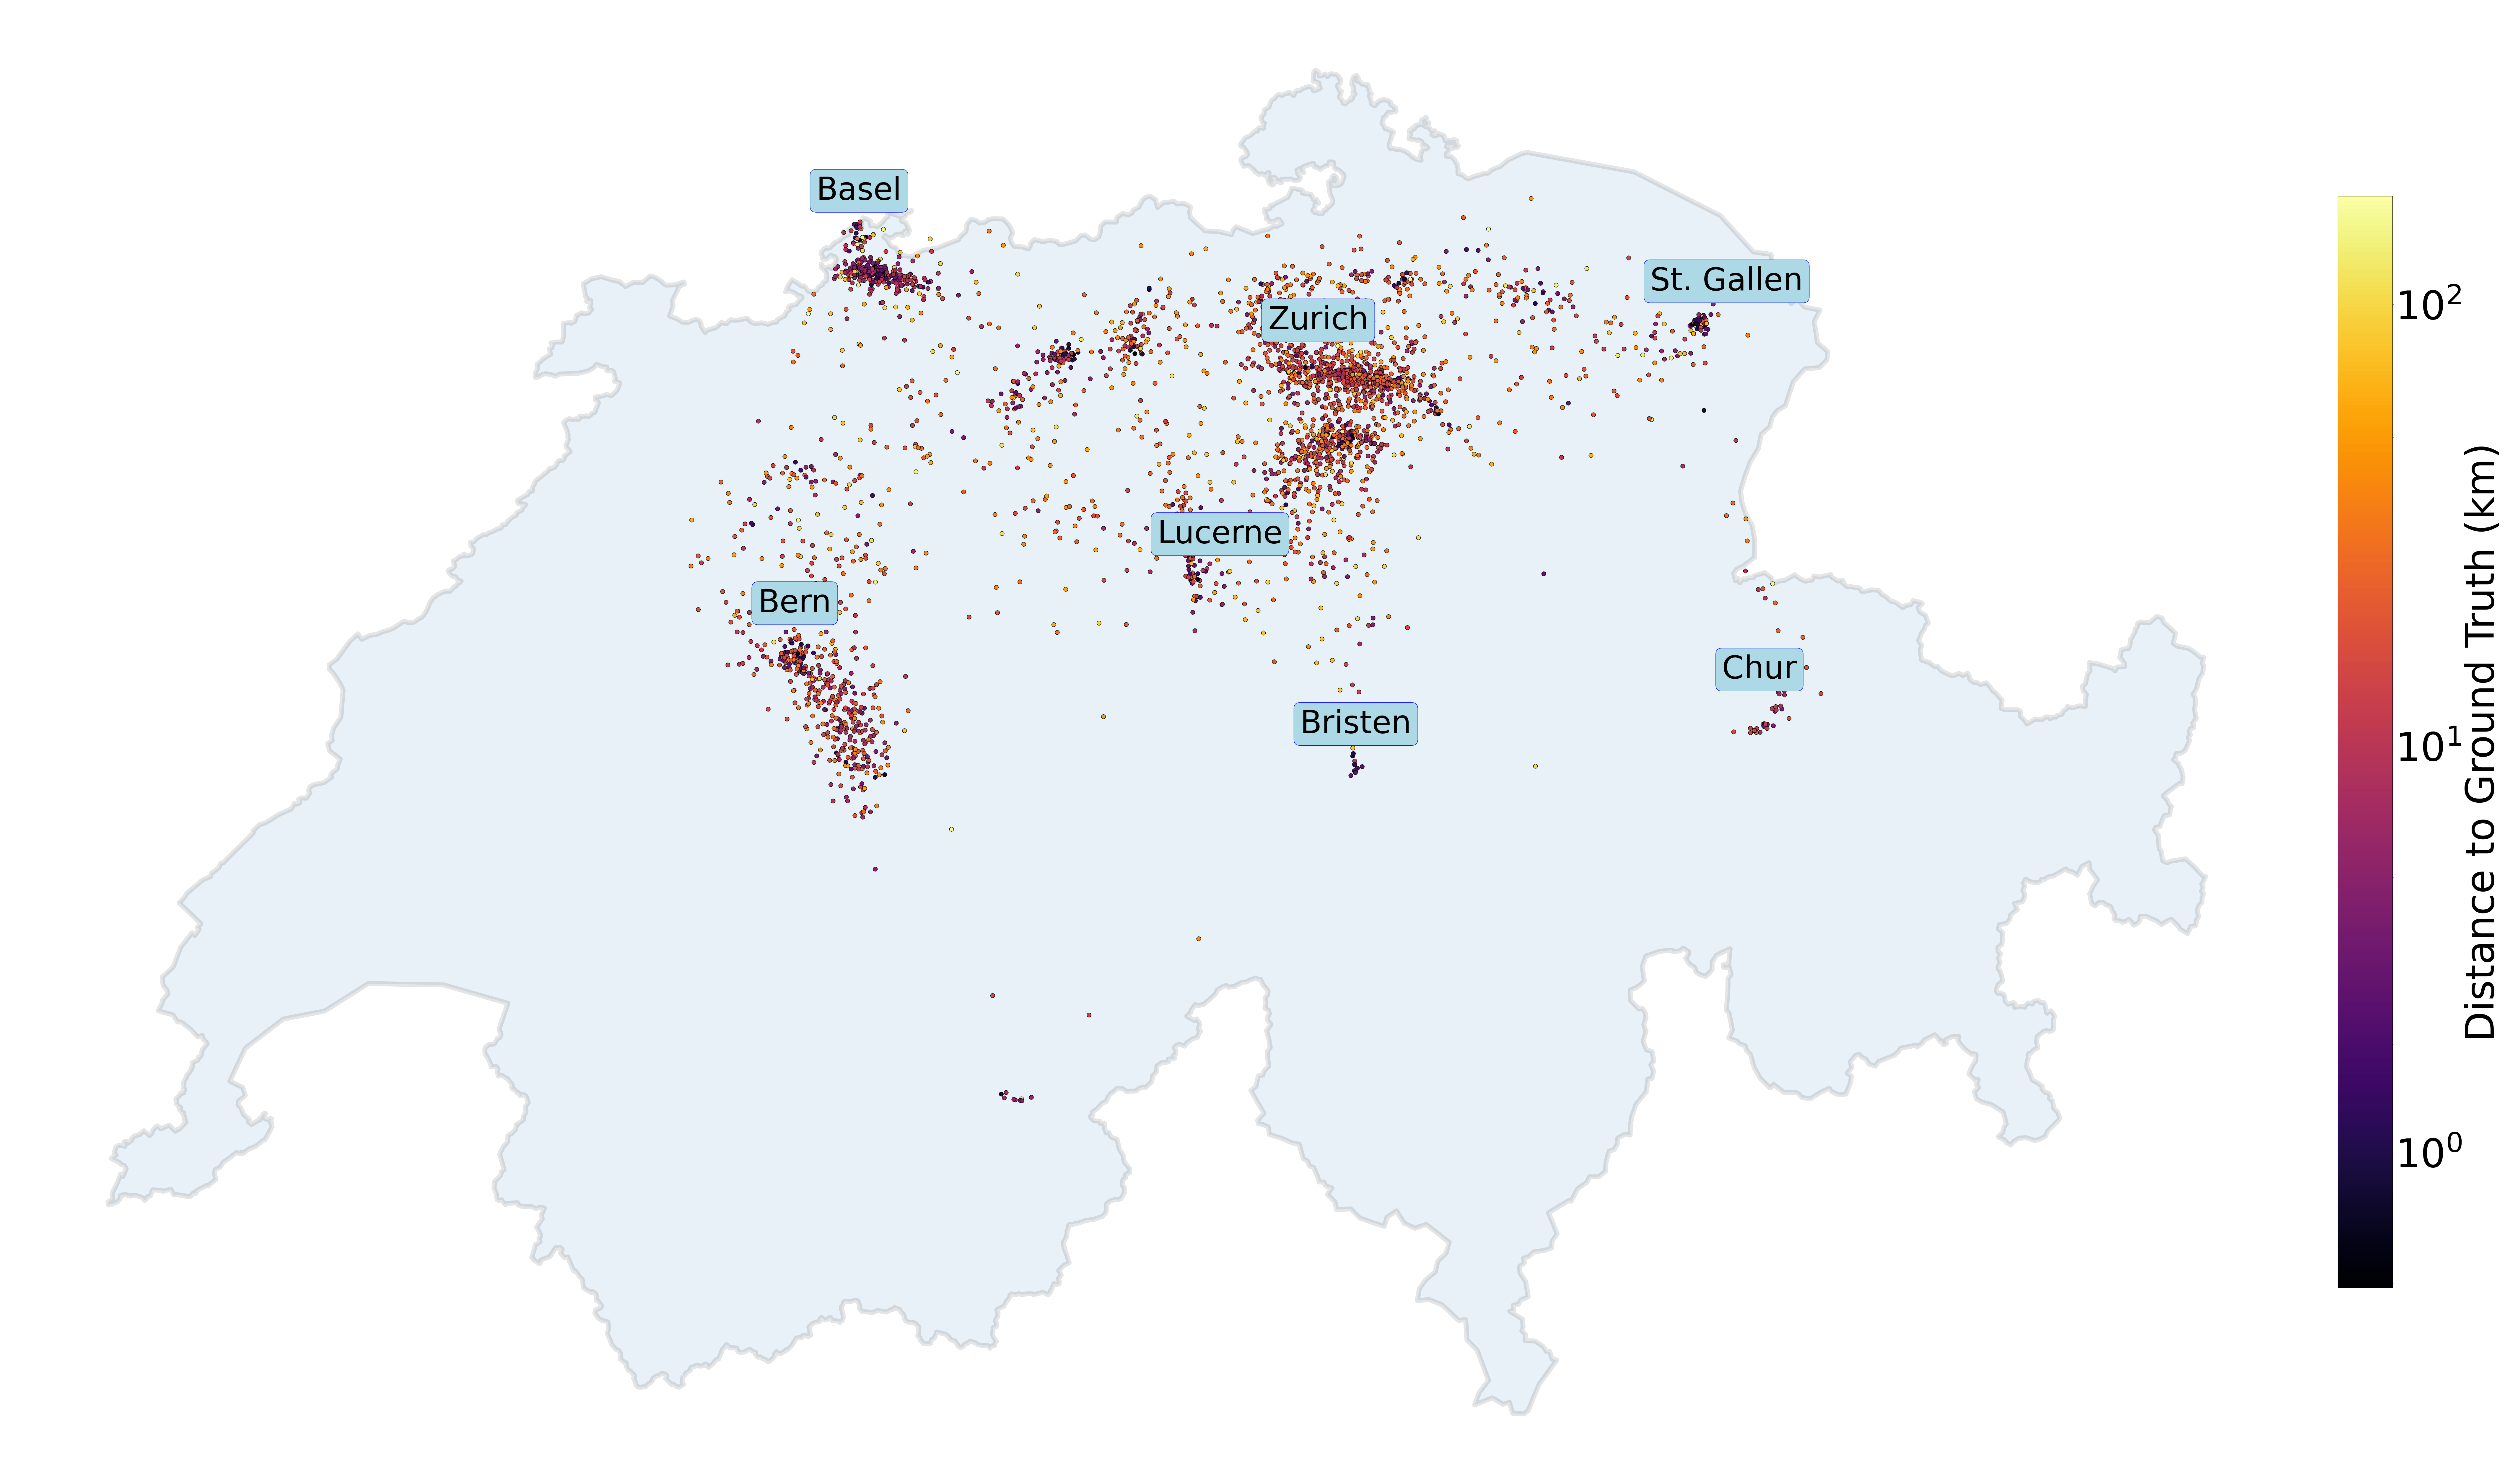
\includegraphics[width=\textwidth]{./figs/dotmap.png}
    \caption{Pointwise distance from the ground truth}
    \label{fig:pointwise-distance}
\end{figure}

\begin{figure}
    \centering
    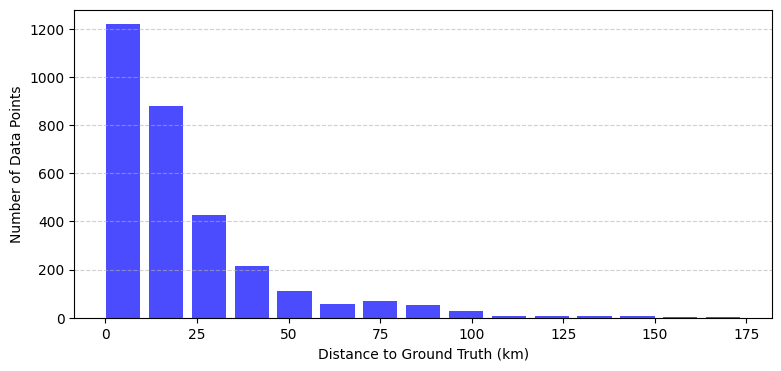
\includegraphics[width=\textwidth]{./figs/barchart.png}
    \caption{Error distribution: distances from predicted locations to ground truth}
    \label{fig:error-distribution}
\end{figure}


\section{Discussion}
\label{sec:Discussion}

\begin{comment}
It is important to include a discussion, which describes what you have learned so far, the merits of the work as well as its limitations.
It can be a separate section or it can appear together with the results or be part of the conclusion).
When evaluating your results, avoid drawing grand conclusions, beyond those that your results can in fact support.
Further, although you may have designed your experiments to answer certain questions,
the results may raise other questions in the eyes of the reader.
It is important that you study the graphs/tables to look for unusual features/entries, and discuss these as well as the main findings.
In particular, carry out an error analysis: b went wrong and why?
\end{comment}

Results show that the Swiss LV95 map projection proved most efficient for predicting geolocation from Swiss Jodel messages. This may indicate that using a metric \gls{acr:crs} like LV95 over a spherical representation like latitude and longitude values can be beneficial in a double regression task for predicting geographical coordinates. It could seem that the model finds it harder to learn spherical representations. These findings are counter to those of \cite[5]{scherrerHeLjuVarDial20202020}, who found that raw latitude and longitude values do not perform worse than metric projections. They only did tests on the UTM projection, however, and did not use the LV95 projection.

Not surprisingly, the language-specific model (\texttt{bert-base-german-cased-finetuned-swiss}) proved most suitable for this task. Being pre-trained on large Swiss corpora, its creators were able to show a 5 percent improvement over its German parent model. It seems this pre-training enhances the model's ability to pick up on dialectal details in the data. The X-Mod-based \texttt{swissbert} model, which is based on a model designed to be multilingual \citep{pfeifferLiftingCurseMultilinguality2022}, did not seem to possess the same dialectal knowledge and performed only marginally better than the German \texttt{bert-base-german-uncased} model.

Furthermore, it is clear from the results that the learning rate schedulers used did not improve the test score. \texttt{ReduceLROnPlateau} and \texttt{OneCycleLR} were tested, and while they greatly reduced the convergence time, they were unable to achieve satisfactory median distances. Since the schedulers showed such little promise for this task, they were not investigated much further. I do think, however, that they could prove efficient if one can find a suitable set of initialization parameters.

Overall, the results are quite good and would suffice for a second place in the VarDial 2020 competition. One would expect, however, that with newer models like \texttt{bert-base-german-cased-finetuned-swiss}, one should be able to achieve better results while using methods similar to those used in 2020. This turned out not to be the case. Pinpointing an exact reason is difficult, but \cite{scherrerHeLjuVarDial20202020} having trained a total of 48 models as opposed to the 15 of this study could be one of them. There may also be some default hyperparameters in the \texttt{simpletransformers} library that \cite{scherrerHeLjuVarDial20202020} did not discuss in their that made it difficult to recreate their results, or there might be other totally different issues with the implementation in this project.

\section{Conclusion and Future Work}
\label{sec:Conclusion}

\begin{comment}
What are the main contributions? How significant are they?
Discuss the contributions in terms of the initial goal formulated in the Introduction.

Also consider how you think the work could be extended or improved, or what you could have done differently.
\end{comment}

\printbibliography

% It is not necessary to include any appendices, but if you do, add them at the very end of the document
%\input{appendices/appendices}

\end{document}
